\Chapter{Reconhecimento de gestos}

Reconhecimento de gestos é uma área da visão computacional na qual uma série de técnicas de processamento de imagens e análise de séries temporais são aplicadas para que o computador consiga `entender' um gesto realizado por um usuário capturado através de câmeras. Diversas aplicações fazem uso dessa área, tais como: Interação entre homem e computador, reconhecimento de linguagens de sinais, navegação e manipulação em ambientes virtuais, jogos fisicamente interativos, detecção de mentiras, etc.

Dois conceitos muito utilizados na literatura na reconhecimento de gestos são os de postura e gesto:

\begin{itemize}
\item \textit{Postura:} Configuração estática do corpo.
\item \textit{Gesto:} Sequência de posturas do corpo dentro de um espaço de tempo.
\end{itemize}

Por exemplo, o gesto de caminhar, envolve uma sequência de posturas como levantar a perna direita, inclinar o corpo levemente para frente, esticar a perna direita, levantar a perna esquerda, etc.

O principal foco desse trabalho são os gestos do corpo, ou seja, baseado-se em uma sequência de posturas, como identificá-la e decidir qual comando deve ser enviado ao computador.


\section{Trabalhos anteriores}

Recentemente, o número de pesquisas de reconhecimento de gestos envolvendo métodos de visão computacional tem crescido.

Um dos trabalhos clássicos em reconhecimento de sequências e um dos pioneiros na utilização de modelos ocultos de Markov para essa tarefa foi desenvolvido por Yamato et al. \cite{YAMATO}, um sistema que reconhece seis jogadas de tennis através de segmentos de vídeos, utilizando malha de características de tamanho \(25\times{25}\), quantização vetorial com codebook de tamanho 72 e seis cadeias de Markov ocultas. A resolução dos vídeos era de \(200\times{200}\) pixels e 256 níveis de cinza e 30 frames/segundo. A taxa de acerto para o jogador \(C\) era de: 100\%, 70.8\%, 66.8\%, 61.2\% no sistemas treinados por vídeos dos jogadores \(C\), \(A + B\), \(B\) e \(A\) respectivamente.

Chen et al. \cite{HandGestureUsingHMMs} criaram um sistema de reconhecimento contínuo de vinte diferentes gestos manuais, utilizando remoção de fundo estático, vetor de características através de descritores Fourier combinados com análise de movimento e modelos ocultos de Markov. O gesto que será reconhecido é avaliado separadamente em cada um dos modelos, sendo o modelo com a maior pontuação o indicador do gesto. Eles obtiveram  uma taxa de identificação acima de 90\%.

Nianjun et al. \cite{EvaluationOfHMMTrainingAlgorithmsForLetterHandGestureRecognition} introduziram uma aplicação que usa visão computacional para reconhecer letras através de gestos reconhecidos da mão do usuário. A mão é segmentada em cada imagem, sua posição é calculada de acordo com o centro da mão e sua trajetória é determinada. Uma suavização é aplicada nessa trajetória e uma sequencia de ângulos do movimento é quantizada para formar uma sequencia discreta. Utilizaram HMMs e os algoritmos de Baum-Welch e Viterbi e o sistema reconhece 26 letras de A a Z, com um banco de dados contendo 30 vídeos para o gesto de cada letra. O taxa de reconhecimento ficou em torno de 90\%.

Truyenque \cite{MestradoTruyenque} em sua tese de mestrado, implementou uma aplicação que utiliza gestos da mão para interagir com slides powerpoint, controlar um jogo simples e desenhar no programa paint, substituindo o mouse. Para isso ele implementou um algoritmo robusto de subtração de fundo estático, funciona bem mesmo com sombras ao redor das detecções, usou autômato finito determinista para representar o processo de inferência dos gestos baseando-se na quantidade de dedos detectados na silhueta. Para detectar um dedo ele construiu uma linha de direção utilizando o método de Mínimos Quadrados descrito por Weisstein \cite{Weisstein}.

Scandaroli e Melo \cite{DeteccaoInterface}, em seu trabalho de conclusão de curso, utilizaram uma câmera USB genérica para detectar
o olhos do usuário após a detecção do rosto dele e então transmitir a posição do usuário em relação a câmera,
fazendo uma câmera no ambiente virtual se movimentar de acordo com a posição dos olhos do usuário. Desenvolveram então um ambiente virtual imersivo,
onde a maneira como o usuário visualizava o ambiente virtual dependia da posição de onde ele olhava para o monitor.
O programa foi desenvolvido utilizando a linguagem C++, auxiliada das bibliotecas OpenCV para processamento de imagem,
OpenGL para desenho do ambiente virtual e Newmat para cálculo de matrizes. Para a detecção do rosto e dos olhos foi utilizado o método de
Viola e Jones \cite{Viola}, baseado em características do tipo Haar utilizando AdaBoost e filtro de Kalman para fazer a correção
e predição da posição da face na imagem. Como resultado o programa rodou a uma taxa de 25 quadros por segundo,
utilizando imagens com resolução 640 por 480 pixels.

Elmezain et al. \cite{HMM-Based_Isolated_Hand_Gesture_Recognition} implementaram um sistema que reconhece gestos com a mão, isolados ou contínuos, através de vídeos, para identificar números de 0 a 9 em tempo real baseados em modelos de Markov. O banco de dados deles armazenava 30 vídeos para cada gesto isolado e 70 vídeos de gestos contínuos, capturados por uma câmera estéreo, com resolução \(240\times{320}\) pixels à 15 quadros/segundo. Eles testaram o sistema utilizando três tipos de topologia diferentes de HMMs, cada uma delas com quantidade de estados variando de 3 a 10. Eles chegaram à conclusão de que a topologia LRB (Left-Right Banded) junto com o algoritmo de Baum-Welch para treinamento e o algoritmo forward com caminho de Viterbi apresentaram a melhor performance.

Pode-se concluir, previo análise de alguns trabalhos relacionados expostos, que o método de segmentação utilizando HMM é o modelo mais apropriado quando se trata de reconhecimento de gestos contínuos, ou como uma sequência de posturas, como o caso de andar, levantar a mão, etc.

\section{Visão Computacional}

Visão computacional é o ramo da ciência da computação que trata de imagens digitais, modificando-a para transformá-la em uma nova representação ou uma decisão. Essas alterações visam objetivos como, por exemplo, avisar se existe uma pessoa numa cena, no caso de decisão. Transformar uma imagem colorida em uma preto-e-branco, no caso de um nova representação. Avisar que um objeto está a uma distância de 1 metro, no caso de informação descritiva.

Em um sistema baseado em visão computacional, o computador recebe uma rede de números de uma câmera ou imagem gravada no disco rígido, esses números muitas vezes revelam pouca informação e contém na ruídos e distorções. Por causa disso, em sistema baseados em visão computacional na prática, outras informações descritivas do ambiente ou outros sensores, precisam ser usados para solucionar essas limitações impostas pelos sensor visual \cite{LearningOpenCV}.

Esse ramo tem crescido muito nos últimos anos porque cada vez mais temos câmera melhores por preços mais acessíveis e computadores com maior poder de processamento. Visão computacional é uma tecnologia com grande potencial para ser integrado a micro-controladores, isso resulta em uma produção em massa muito mais fácil e barata do que outros dispositivos com partes mecânicas como luvas ou roupas especiais.

Quando se trata de utilizar visão computacional em interação humano/computador, é importante que a interação aconteça em tempo real, ou seja, a latência (\textit{delay}) entre as modificações no ambiente real e suas adaptações na representação virtual devem ser minimizadas ao máximo possível \cite{MestradoTruyenque}.

Sistemas que reconhecem gestos e movimentos, geralmente passam por um fluxo processamento na seguinte ordem; obtenção de uma imagem ou uma sequência delas através de uma câmera ou vídeo digital, o pré-processamento dessas imagens, aplicando uma série de métodos que melhoram e preparam a imagem para ter informações importantes extraídas dela.

Com as imagens tratadas, o processo de extração de características acontece, nele a imagem sofre uma análise em busca de padrões numéricos de interesse, que representem com capacidade a imagem. Um vetor de características é criado com esses valores e a partir desses vetores, algoritmos de reconhecimento de padrões são aplicados para determinar à que grupo, dentre os possíveis, essa imagem pertence.

\subsection{Características para reconhecimento de posturas}

Uma característica em uma imagem é uma mínima quantidade de informação, preferencialmente numérica, que a descreve. Para que essa característica seja bem representativa, uma forma eficiente de caracterização é fundamental no processo de reconhecimento de gestos, já que gestos apresentam muitos detalhes e variações no que se diz respeito a forma, movimento e texturas. 

Existem diversos métodos de extrair características, entre eles, transformada de Fourier, transformada discreta de cosseno, momentos invariantes, malha de características, cores, características geométricas (contornos, orientação,número de interseções, etc), direção do movimento são exemplos de características que podem ser utilizadas. A dificuldade muitas vezes é encontrar características que não deixem de estar disponíveis devido as condições de iluminação (pouca ou muita luz) \cite{Vision-Based-Gesture-Recognition-A-Review} e \cite{DCT}.

Para selecionar características eficientes e precisas, alguns critérios são considerados úteis como; características devem ser escolhidas de forma que elas não se repliquem, ou seja, duas imagens diferentes não deveriam ter as mesmas características. Elas devem ser facilmente computadas, para que possamos trabalhar com resultados em tempo real e ela devem preferencialmente serem invariantes em relação a rotação, translação e escala \cite{HandGestureUsingHMMs}.



\section{Processo de Classificação}

No reconhecimento dos gestos, será necessário identificar as posturas, que são imagens estáticas dos gestos e caracterizá-las, para que então elas possam ser agrupadas de acordo com suas semelhanças e descritas dentro de um conjunto finito de possibilidades. Um método de reconhecimento de padrões é imprescindível nesse processo.

Um gesto é uma sequência de posturas em um espaço de tempo. Os gestos também precisam ser agrupados de acordo com suas semelhanças. A cada espaço de tempo selecionado o sistema precisa então identificar uma sequência de posturas e dada essa sequência, responder qual o gesto mais provável foi executado. Um modelo que torne possível lidar com informações sequenciais será obrigatório.

\subsection{Cadeias Ocultas de Markov}
\label{hmm}

Processos Markovianos são um tipo especial de processos estocásticos. Um processo estocástico é dito Markoviano se dada uma sequência temporal de realizações, a probabilidade desse processo passar para um estado qualquer dentro do espaço de amostras no próximo instante  depende única e exclusivamente do estado corrente no qual o sistema se encontra, ou seja, a probabilidade do passo seguinte, de \(X_{t-1}\) para \(X_t\), depende apenas do estado de origem desse passo, \(X_{t-1}\). Essa propriedade é conhecida como \textit{Markov property} (propriedade Markoviana).

Na maioria dos processos Markovianos, cada estado corresponde a algo que possa ser observado, como por exemplo, uma moeda jogada que cai para com a face para cima apresenta dois resultados observáveis, cara ou coroa. Cadeias ocultas de Markov, também conhecidas como modelos de Markov ocultos, são utilizadas para modelos de processos Markovianos que geram observáveis de forma indireta, de acordo com as transições entre os estados da cadeia de Markov que governam o processo, mas que não podem ser diretamente observadas. Em outras palavras, a progressão do modelo está escondida do observador e a observação é indireta, feita por inferência, pois os observáveis são funções probabilísticas dos estados da cadeia ou das transições entre esses estados. Dessa forma não é possível saber exatamente qual caminho ou sequência que levaram a determinada observação \cite{HMMLuciana}.

Segundo Rabiner \cite{Rabiner}, uma HMM é simbolicamente descrita por: \[ \lambda = (A, B, \pi), \] e caracterizada pelos seguintes elementos:

\begin{itemize}
\item \( E = \{ E_1,E_2,...,E_N \} \): Conjunto de \(N\) estados.
\item \( S = \{ S_1,S_2,...,S_M \} \): Conjunto de \(M\) símbolos observáveis por estado.
\item \(A = [a_{ij}]_{N\times{N}} \): Matriz de distribuição de probabilidades de transições de estados.
\item \(B = \{ b_{ij} \}_{N\times{M}}\): Matriz de distribuição de probabilidades de observação dos símbolos.
\item \(\pi = \{ \pi_{i} \}_N \): Vetor de distribuição inicial de estados.
\end{itemize}

A condição de soma das saídas de cada estado é \( \Sigma_{j=1} a_{ij}=1\), para $i=1,...,N$ e \( \Sigma_{j=1} b_{ij}=1\), para $i=1,...,M $. A Figura \ref{img:HMM_exemplo} mostra uma HMM \( \lambda = (A, B, \pi)\) para $N=3$ e $M=3$.

\begin{figure}[!htbp]
  \centering
  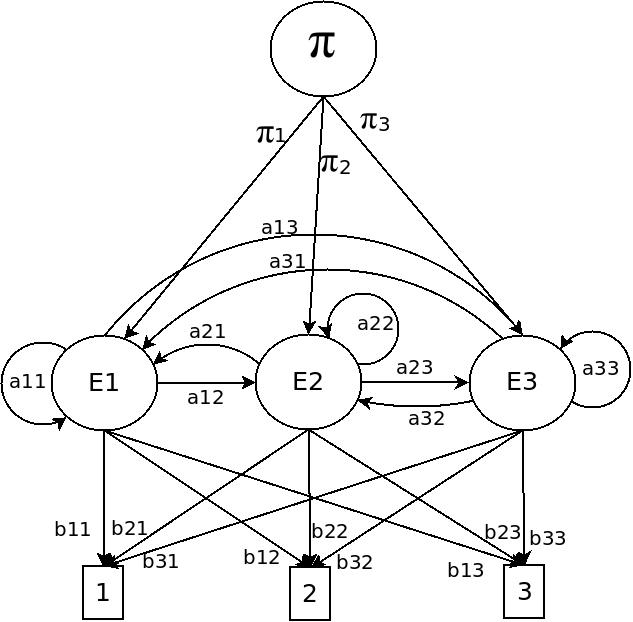
\includegraphics[scale=0.40]{imagens/HMM_exemplo.jpg}
  \caption{Grafo de um Modelo Oculto de Markov (HMM).}
  \label{img:HMM_exemplo}
\end{figure}

Existem três tipos de topologia na hora da modelagem de HMMs:

\begin{itemize}
\item \textbf{Totalmente conectada (\textit{Ergodic model}):} Todos os estados pode ser alcançado de todos os outros estados.
\item \textbf{\textit{Left-Right} (LR):} Cada estado pode voltar para si ou ir para todos os estados seguintes.
\item \textbf{\textit{Left-Right Banded} (LRB):} Cada estado pode voltar para si ou ir apenas para um estado sucessor seguinte.
\end{itemize}

A Figura \ref{img:topologias_hmm} demonstra um exemplo de grafo dessas topologias.

\begin{figure}[!htbp]
\centering
\subfigure[\textit{Ergodic model}]{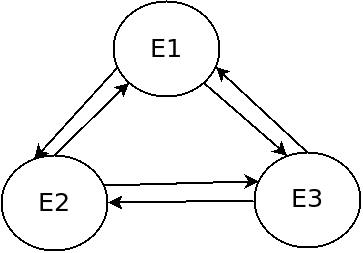
\includegraphics[width=5cm]{imagens/ergodic_HMM.jpg}}
\subfigure[\textit{Left-Right}]{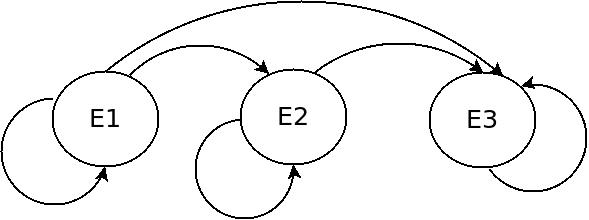
\includegraphics[width=7cm]{imagens/LR_HMM.jpg}}
\subfigure[\textit{Left-Right Banded}]{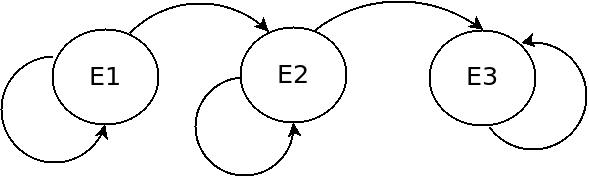
\includegraphics[width=7cm]{imagens/LRB_HMM.jpg}}
\caption{Modelos de topologias HMM.}
\label{img:topologias_hmm}
\end{figure}

Durante o processo de reconhecimento sequências de observáveis serão armazenadas para serem avaliadas em diferentes HMMs, essas sequências representam os gestos que o usuário executa diante da câmera. Para que esses gestos possam ser identificados é preciso que o sistema solucione 3 problemas: Qual a probabilidade de um gesto pertencer a uma determinada HMM, se uma gesto pertence a uma HMM qual a sequência de estados na HMM que tem a maior chance de produzi-lo e por último como estimar os parâmetros de uma HMM de forma que ela apresente a melhor probabilidade de produzir determinados tipos de gestos. Esses 3 problemas são definidos na literatura como: 

\begin{itemize}
\item \textbf{Problema 1:} Probabilidade de uma Sequência de Observáveis; como calcular de forma eficiente a probabilidade de uma sequência ser gerada por um modelo?
\item \textbf{Problema 2:} Sequência Ótima de Estados; dentre todas as diferentes sequências de estados que poderiam ter gerado uma sequência, qual é a mais provável?
\item \textbf{Problema 3:} Maximização da Probabilidade de uma Sequência de Observáveis; quais os melhores parâmetros \( \lambda = (A, B, \pi) \) do modelo para maximizar a probabilidade de uma sequência \(S\), \(P(S|\lambda)\)?
\end{itemize}

Os dois primeiros problemas podem ser resolvidos pelo algoritmo de Viterbi, o terceiro problema pode ser solucionado utilizando-se do algoritmo de Baum-Welch.


\subsection{Algoritmo de Viterbi}

Esse algoritmo é usado na resolução do problema de encontrar a sequência ótima de estados associada à seguência de observáveis. Segundo Rabiner \cite{Rabiner} é difícil decidir um critério de otimização, dentre vários que possam existir. Dessa forma a resolução desse problema poderia se dar de diferentes formas e diferentes sequências supostamente ótimas, de acordo com o critério de otimização escolhido.

 O algoritmo de Viterbi é uma solução ótima recursiva para estimar a sequência de estados em um processo de Markov de estado finito e tempo discreto. Encontrar a sequência de estados mais provável,\( E = E_1,E_2,...,E_T \), dada uma sequência de símbolos \( S = S_1,S_2,...,S_T \), ou seja, maximizar \( P(E|S,\lambda) \) equivale a maximizar \( P(E,S|\lambda) \). Ambas operações vão devolver a sequência mais provável de estados.

 Esse algoritmo funciona multiplicando os pesos das arestas anterior e próxima ao estado atual, obtendo assim sequências parciais mais prováveis. Uma escolha arbitrária acontece quando duas sequências apresentam a mesma probabilidade. Maiores informações podem ser encontradas no trabalho de Rabiner \cite{Rabiner} ou Espindola \cite{HMMLuciana}., onde o algoritmo de Viterbi para HMM é formulado. Diferentes trabalhos relacionados com o tema tiveram influência.

\subsection{Algoritmo de Baum-Welch}

Segundo \cite{Rabiner} esse é o problema mais difícil, entre os três problemas fundamentais, de resolver, porque não existe método analítico que permita que os parâmetros \( \lambda = (A, B, \pi) \) que maximizam a probabilidade de um modelo gerar uma sequência completa de símbolos observáveis, \( P(S|\lambda) \).

Contudo, o algoritmo de Baum-Welch resolve esse problema maximizando a probabilidade local. Diversos somatórios são realizados sobre o tempo de observação, $T$, com o intuito de se obter estimativas do número de vezes que cada estado é visitado em todo esse período.

Maiores detalhes como as formalizações matemáticas e o algoritmo podem ser encontrados nas obras de Rabiner \cite{Rabiner} ou Espindola \cite{HMMLuciana}.

